%%%%%%%%%%%%%%%%%%%%%%%%%%%%%%%%%%%%%%%%%%%%%%%%%%%%%%%%%%%%%%%
%
% Welcome to Overleaf --- just edit your LaTeX on the left,
% and we'll compile it for you on the right. If you open the
% 'Share' menu, you can invite other users to edit at the same
% time. See www.overleaf.com/learn for more info. Enjoy!
%
%%%%%%%%%%%%%%%%%%%%%%%%%%%%%%%%%%%%%%%%%%%%%%%%%%%%%%%%%%%%%%%
\documentclass[9pt]{beamer}
\usepackage{tikz}
\usetikzlibrary{positioning}
\usepackage{graphicx}
\usepackage{caption}
\setbeamertemplate{caption}[numbered]

\usetheme{Madrid}
\usecolortheme{default}

%Information to be included in the title page:
\title{Application of Neural Network Approach to Numerical Integration}
\author{Gregory A. Shipunov, student of gr. 4181\inst{1} \\ supervisors: Oksana I. Streltsova,\inst{1, 2} Yury L. Kalinovsky\inst{1, 2}}
\institute{
    \inst{1} Dubna State University, 19 Universitetskaya St, Dubna, 141980, Russian Federation \\
    \inst{2} Joint Institute for Nuclear Research, 6 Joliot-Curie St, Dubna, 141980, Russian Federation
}
\date{}

\newcommand{\logoLeft}[1]{
    \begin{tikzpicture}[remember picture,overlay]
        \node[anchor=north west, inner sep=0pt] at (current page.north west) {\includegraphics[width=2cm]{#1}};
    \end{tikzpicture}
}

\newcommand{\logoRight}[1]{
    \begin{tikzpicture}[remember picture,overlay]
        \node[anchor=north east, inner sep=0pt] at (current page.north east) {\includegraphics[width=2cm]{#1}};
    \end{tikzpicture}
}

\newcommand{\logoBottomLeft}[1]{
    \begin{tikzpicture}[remember picture,overlay]
        \node[anchor=south west, inner sep=10pt, yshift=0.4cm, xshift=-0.1cm] at (current page.south west) {\includegraphics[width=1.5cm]{#1}};
    \end{tikzpicture}
}

\newcommand{\logoBottomRight}[1]{
    \begin{tikzpicture}[remember picture,overlay]
        \node[anchor=south east, inner sep=0pt, yshift=0.7cm] at (current page.south east) {\includegraphics[width=2cm]{#1}};
    \end{tikzpicture}
}

\setbeamertemplate{footline}[page number]

\AtBeginSection[]
{
  \begin{frame}
    \frametitle{Table of Contents}
    \tableofcontents[currentsection]
  \end{frame}
}
%------------------------------------------------------------


\begin{document}

\frame{
    \titlepage
    \logoLeft{logo_new_small_eng.png}  
    \logoRight{logo_jinr_21.jpg} 
    \logoBottomLeft{isau.pdf} 
    \logoBottomRight{mlit.png}
    \begin{tikzpicture}[remember picture,overlay]
        \node[anchor=south, yshift=0.7cm] at (current page.south) {2025};
    \end{tikzpicture}
}

\begin{frame}
\frametitle{Table of Contents}
\tableofcontents
\end{frame}

\section{Problem Statement}

\begin{frame}{Problem Statement 1}
This work is dedicated to developing the software for numerical calculations in domain of modelling of physical processes for NICA collider. Numerical modeling of physical processes involves studying of the particle properties based on Bethe-Salpeter equation:

\begin{eqnarray}\label{BS}
  \Gamma (q,P) = -\frac{4}{3} \int \frac{d^4 p}{(2\pi)^4}
  D(q-p) \gamma_\alpha S_1 \Gamma (q,P)
S_2 \gamma_\alpha .
\end{eqnarray}

The vertex function $\Gamma (p,P)$ depends on the relative
momentum $p$, and the total momentum of the bound state $P$. 
$S_i(p)$ are the dressed quark propagator in the Euclidean space: 
\begin{equation}\label{Eqn:q_prop}
S_i(p_i)=\frac{1}{i (p_i\cdot \gamma) + m_i}
\end{equation}
The momenta $p_i=p+q_i$, $q_i = b_i P$, $i=1,2$ with 
$b_1 =- m_1/(m_1+m_2)$, $b_2 = m_2/(m_1+m_2)$, $m_i$ are the constituent quark masses. 

\end{frame}

\begin{frame}{Problem Statement 2}
Equation (\ref{BS}) contains the interaction kernel $D(q-p)$ 
which describes the effective gluon interaction within a meson. 
We consider the rank -1 separable  model 
\begin{eqnarray}\label{kernel}
  D(q-p) = D_0 F(q^2) F(p^2) \, ,
\end{eqnarray}
where $D_0$ is the coupling constant and the function 
$F(p^2)$ is related to scalar part of Bethe - Salpeter  vertex
function. We employ  $F(q^2)$  in the Gaussian form 
$F(p^2)= e^{-p^2/\lambda^2}$ with the parameter $\lambda$ which  characterizes the finite size of the meson. 

\end{frame}

\begin{frame}{Problem Statement 3}

This separable Anzatz of the interaction kernel (\ref{kernel}) allows to write the meson observables in the term of the polarization operator (the buble diagram): 

\begin{equation}
        \tikz[baseline=-0.5ex]{
        \filldraw (0, 0) circle (0.1cm);
        \filldraw (1, 0) circle (0.1cm);
        \draw[->, thick] (0.1, 0.05) to[out=45, in=135] (0.9, 0.05);
        \draw[<-, thick] (0.1, -0.05) to[out=-45, in=-135] (0.9, -0.05);
    } + \tikz[baseline=-0.5ex]{
        \filldraw (0, 0) circle (0.1cm);
        \filldraw (1, 0) circle (0.1cm);
        \draw[->, thick] (0.1, 0.05) to[out=45, in=135] (0.9, 0.05);
        \draw[<-, thick] (0.1, -0.05) to[out=-45, in=-135] (0.9, -0.05);
    }\tikz[baseline=-0.5ex]{
        \filldraw (0, 0) circle (0.1cm);
        \filldraw (1, 0) circle (0.1cm);
        \draw[->, thick] (0.1, 0.05) to[out=45, in=135] (0.9, 0.05);
        \draw[<-, thick] (0.1, -0.05) to[out=-45, in=-135] (0.9, -0.05);
    } + ... = \frac{1}{1 - \tikz[baseline=-0.5ex]{
        \filldraw (0, 0) circle (0.1cm);
        \filldraw (1, 0) circle (0.1cm);
        \draw[->, thick] (0.1, 0.05) to[out=45, in=135] (0.9, 0.05);
        \draw[<-, thick] (0.1, -0.05) to[out=-45, in=-135] (0.9, -0.05);
    }},
\end{equation}
where 
\begin{equation}
        \tikz[baseline=-0.5ex]{
        \filldraw (0, 0) circle (0.1cm);
        \filldraw (1, 0) circle (0.1cm);
        \draw[->, thick] (0.1, 0.05) to[out=45, in=135] (0.9, 0.05);
        \draw[<-, thick] (0.1, -0.05) to[out=-45, in=-135] (0.9, -0.05);
    } \to \int_{0}^{\infty}\frac{dp}{2\pi^4}F(p^2)\frac{1}{[(p + q_1)^2 + m_1^2][(p + q_2)^2 + m_2^2]}.
\end{equation}

To calculate these integrals we use the equations:

\begin{equation}
    \frac{1}{(p + q_i)^2 + m_i^2} = \int_{0}^{\infty}dt\{\exp(-t[(p + q_i)^2 + m_i^2])\}, 
\end{equation}
\begin{equation}
    F(p^2) = \int_{0}^{\infty}ds\{\exp(-sp^2)F(s)\} .
\end{equation}

The case of more than two mesons is described using triple and quadruple integrals.

\end{frame}

\begin{frame}{Problem Statement 4}

This way the following integral equation is produced:
\begin{equation}
    \label{eq:the-integral}
    \int_{0}^{1}d\alpha\{\alpha^{a}(1 - \alpha)^b\}\int_{0}^{\infty}dt\{\frac{t^m}{(1+t)^n}F[z_{0}]\} \equiv I(a, b, m, n; F[z_{0}]),
\end{equation}
\begin{equation*}   
    F[z_0] = \exp(-2z_0),
\end{equation*}
\begin{equation*} 
    z_0 = tD + \frac{t}{1 + t}R^2,
\end{equation*}
\begin{equation*}     
    D = \alpha_1(b_1^{2}P^2 + m_1^2) + \alpha_2(b_2^{2}P^2 + m_2^2),
\end{equation*}
\begin{equation*} 
        R^2 = (\alpha_1^{2}b_1^2 + \alpha_2^{2}b_2^2 + 2\alpha_{1}\alpha_{2}b_{1}b_2)P^2,
\end{equation*}
\begin{equation*} 
    b_1 = -\frac{m_1}{m_1 + m_2},
    b_2 = \frac{m_2}{m_1 + m_2},
\end{equation*}
\begin{equation*}
    \alpha_1 = \alpha, \alpha_2 = 1 - \alpha.
\end{equation*}

%\begin{figure}
%    \centering
%    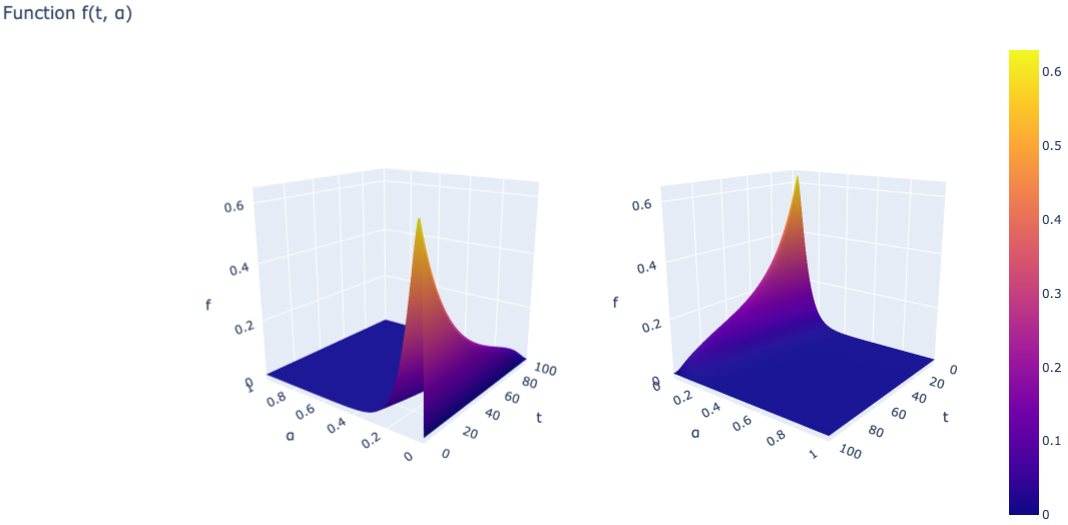
\includegraphics[width=0.8\linewidth]{f(t,a)33.png}
%    \caption{Integrand function (\ref{eq:the-integral}) plot - view from (0, 0, 0) and (100, 0, 0) corners}
%    \label{fig:integrand-plot}
%\end{figure}

\noindent This integral is used in multiple calculations in the problem and its value describes the form of the mesons. The calculations require multiple (50 times and more) integrations of (\ref{eq:the-integral}).
    
\end{frame}

\begin{frame}{Problem Statement 5}

Let a continuous real function $f(\mathbf{x})$ be defined as $f: {\rm I\!R}^n \to {\rm I\!R}$. Let $\Omega$ be a compact subset of ${\rm I\!R}^n$ and let $G$ be a bounded convex subset of $\Omega$. Let, also, $\mathbf{x}$ be a vector of $n$ dimensions in $\Omega$. Than

\begin{equation}
    \label{eq: integral definition}
    I(f) = \int_G d\mathbf{x} f(\mathbf{x}),
\end{equation}

\noindent is a definite integral of $f$ across set $G$. 

Therefore, the problem is to get the $I(f)$ value calculated with use of neural network approach. The neural network model will be used to approximate the function $f(\mathbf{x})$\footnote{S. Lloyd, R. A. Irani, M. Ahmadi, Using neural networks for fast numerical integration and
optimization, IEEE Access 8 (2020) 84519–84531.}. Than this model will be used to calculate the approximate integral value:

\begin{equation}
    \label{eq: integral definition}
    \hat{I}(f) = \int_G d\mathbf{x} \hat{f}(\mathbf{x}),
\end{equation}

\end{frame}

\begin{frame}{Problem Statement 6}

\begin{figure}[h!]
    \centering
    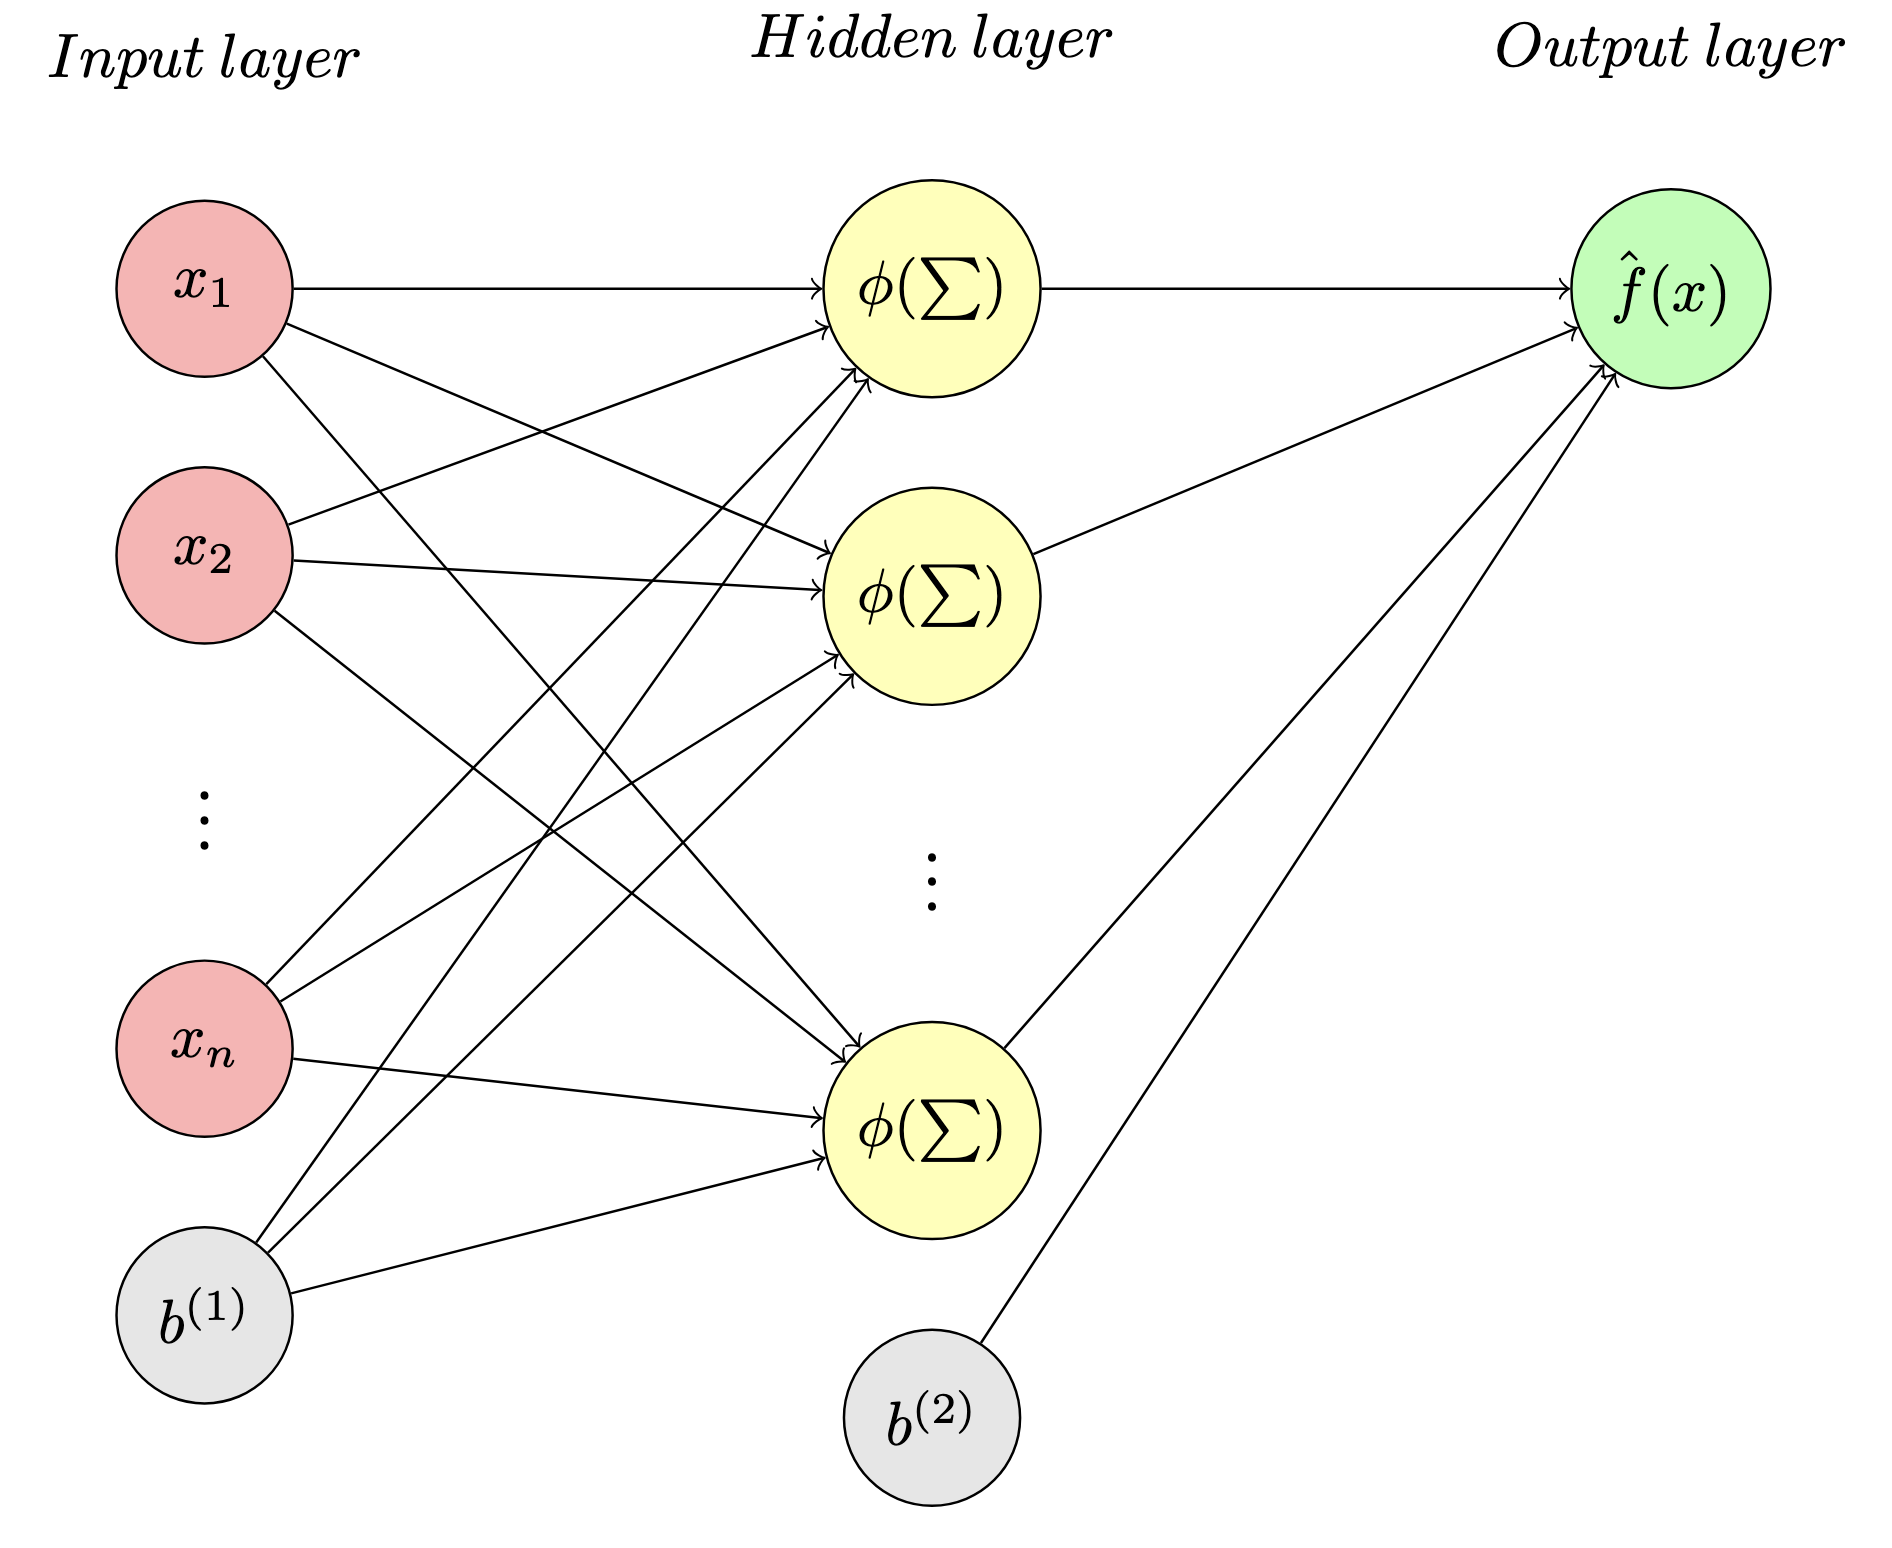
\includegraphics[width=0.4\linewidth]{structre-as-photo.png}
    \caption{The MLP structure used in the neural network approach}
    \label{fig:structure}
\end{figure}

The MLP structure will have logistic sigmoid as activation function on the hidden layer:

\begin{equation}
    \label{eq:sigmoid}
    \phi(z) = \frac{1}{1+\exp(-z)}.
\end{equation}

\end{frame}

\begin{frame}{Problem Statement 7}

\noindent With $\phi(z)$ defined, network structure's mathematical form is:

\begin{equation}
    \label{eq:math-form-mlp}
    \hat{f}(x) = b^{(2)} + \sum_{j=1}^{k}w_j^{(2)}\phi(b_j^{(1)}+\sum_{i=1}^{n}w_{ji}^{(1)}x_{i}).
\end{equation}

We can apply following substitution\footnote{S. Lloyd, R. A. Irani, M. Ahmadi, Using neural networks for fast numerical integration and
optimization, IEEE Access 8 (2020) 84519–84531.} here:

\begin{equation}
    \label{eq:substitution-li-sigm}
    -Li_0(-\exp(z)) = \frac{1}{1+\exp(-z)} = \phi(z),
\end{equation}

\noindent where $Li_0(u(z))$ is a Jonquière's function or the polylogarithm of order 0.
    
\end{frame}

\begin{frame}{Problem Statement 8}

Let number of dimensions $n = 1$. With substitution (\ref{eq:substitution-li-sigm}) equation (\ref{eq:math-form-mlp}) can be integrated over given boundaries $[\alpha, \beta]$ to produce the following numerical integration formulae for 1-dimensional case\footnote{S. Lloyd, R. A. Irani, M. Ahmadi, Using neural networks for fast numerical integration and
optimization, IEEE Access 8 (2020) 84519–84531.}:

\begin{equation*}
\hat{I}(f) = \int_{\alpha}^{\beta} dx \left(b^{(2)} + \sum_{j=1}^{k}w_j^{(2)}\phi(b_j^{(1)} + w_{1j}^{(1)}x) \right) =
\end{equation*}
\begin{equation}
= b^{(2)}(\beta - \alpha) + \sum_{j=1}^{k}w_j^{(2)} \left( (\beta - \alpha) + \frac{\Phi_j}{w_{1j}^{(1)}} \right),
\label{eq:numerical_method_1}
\end{equation}
\begin{equation}
\label{eq:numerical_method_last}
\Phi_j = Li_1(-\exp[-b_j^{(1)}-w_{1j}^{(1)}\alpha]) - Li_1(-\exp[-b_j^{(1)}-w_{1j}^{(1)}\beta]).
\end{equation}
Formulae (\ref{eq:numerical_method_1}-\ref{eq:numerical_method_last}) can be extrapolated to higher dimensions.

Thus we have got the numerical integration method.

\end{frame}

\section{Results}

\begin{frame}{Results 1}

\begin{figure}[h!]
    \centering
    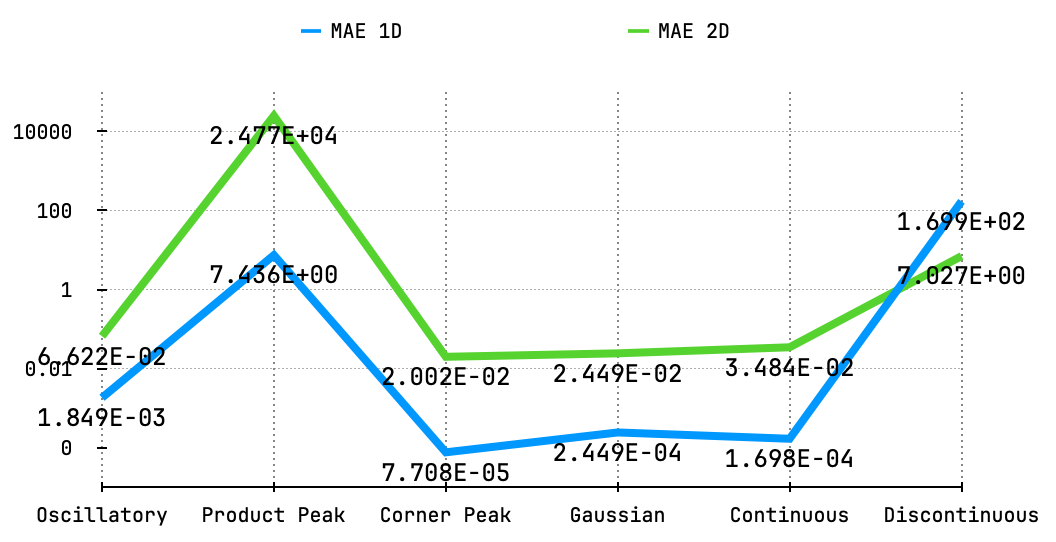
\includegraphics[width=0.7\linewidth]{maes.png}
    \caption{The MAE between neural network numerical integration values and quad numerical integration values}
    \label{fig:maes}
\end{figure}

Figure \ref{fig:maes} depicts the mean absolute errors of integration of Alan Genz's package\footnote{A. Genz, Testing multidimensional integration routines, in: Proc. of international confer-
ence on Tools, methods and languages for scientific and engineering computation, 1984, pp.
81–94.} 1D and 2D functions compared to results calculated using \textit{scipy.integrate.quad} fucntion of Python programming language. The neural network model had hidden layer size was k = 100. 
    
\end{frame}

\begin{frame}{Results 2}

\begin{figure}[h!]
    \centering
    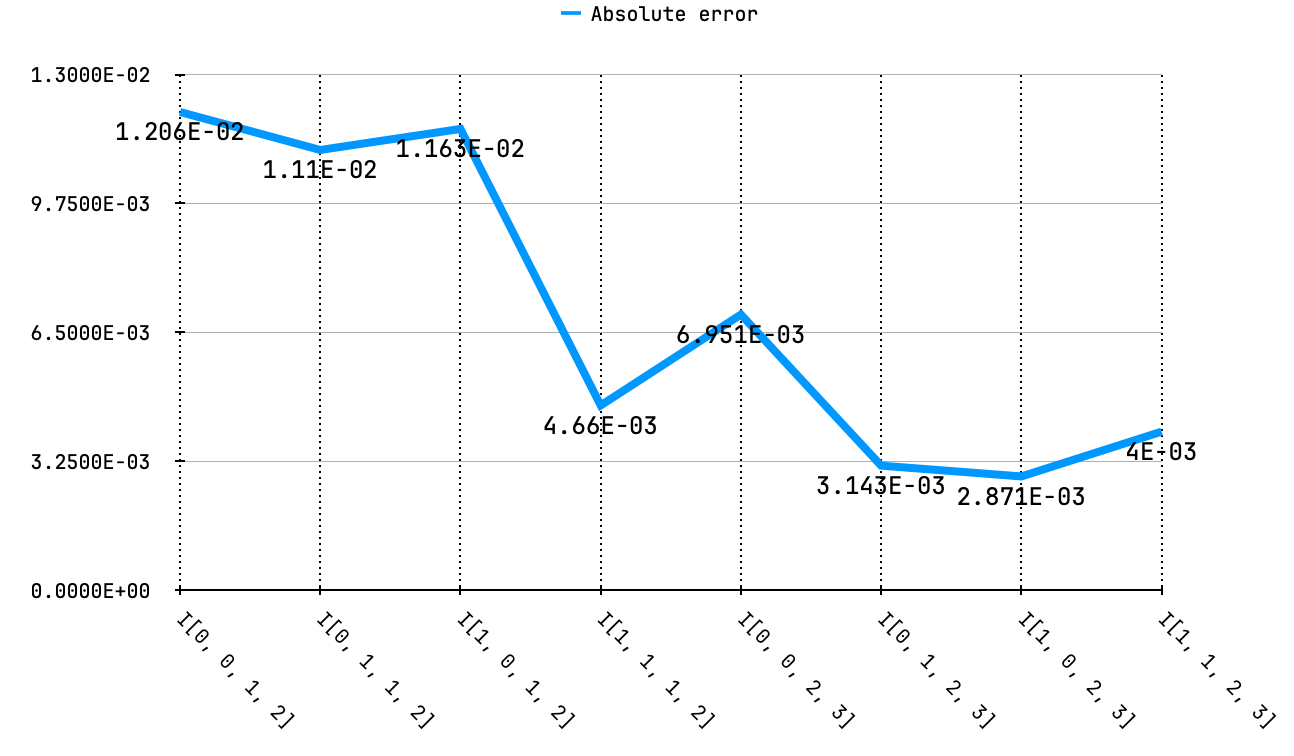
\includegraphics[width=0.7\linewidth]{iaes.png}
    \caption{The absolute errors between numerical integral values calculated using neural network approach and FORTRAN function qdag}
    \label{fig:iaes}
\end{figure}

Figure \ref{fig:iaes} depicts the absolute errors of integration of equation (\ref{eq:the-integral}) compared to results calculated previously using \textit{qdag} function of FORTRAN programming language. The neural network model had hidden layer size was k = 100.
    
\end{frame}

\section{Benefits of using neural network approach}

\begin{frame}{Benefits of using neural network approach}

\begin{itemize}
    \item The integration of similar function across different boundaries time efficiency.
    \item The integration of functions of high-dimensions.
\end{itemize}
    
\end{frame}

\section{Future plans}

\begin{frame}{Future plans}

\begin{itemize}
    \item Improve accuracy of integration.
    \item Implement higher dimensions numerical integration functionality.
    \item Consider other ways to use neural networks for numerical integration.
\end{itemize}
    
\end{frame}

\begin{frame}
  \centering
  \vspace{1cm}
  \Large Thank You for Your Attention!
\end{frame}

\end{document}
